\documentclass[12pt, titlepage, oneside]{article}

\usepackage[margin=0.5in]{geometry}

\usepackage{siunitx, booktabs, amsmath, enumitem, pdfpages,mathrsfs,tabularx,caption, graphicx, pgfplots, textcomp,wrapfig, commath, svg}

\usepackage{parskip}

\usepackage[siunitx]{circuitikz}
\sisetup{detect-weight=true, detect-family=true}

\setlength\parindent{0pt}

\let\oldhat\hat
\let\oldvec\vec
\newcommand{\cross}{\bm{\times}}
\renewcommand{\hat}[1]{\oldhat{\mathbf{#1}}}

\usepackage{bm}
\renewcommand{\vec}[1]{\oldvec{\bm{#1}}}
\renewcommand{\hat}[1]{\oldhat{\bm{#1}}}
\renewcommand{\b}[1]{\textbf{#1}}

\newcommand{\de}[1]{\noindent\fbox{\parbox{\textwidth}{#1}}}

\newcommand{\be}{\begin{equation*}}
\newcommand{\ee}{\end{equation*}}

\begin{document}

\setcounter{section}{3}
\setcounter{page}{10}

\section{Conditional Probability}

Probabilities do not live in a vacuum. They are determined by information available, for instance how an experiment is carried out. Some times additional information is available that changes the probability.

$P(B|A)$ is the conditional probability of $B$ given the knowledge that event $A$ occurs.

\de{

\b{Example 2.22} 400 items are classified by surface flaws and as defective.

\begin{center}
  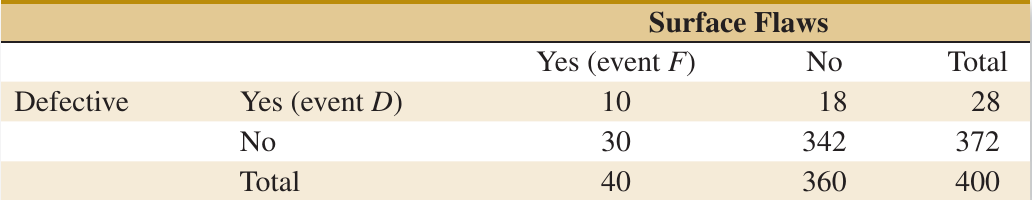
\includegraphics[scale=0.35]{1.png}
\end{center}

Notice the following,
\begin{align*}
  P(D) = \frac{28}{400} \\[2mm]
  P(D|F) = \frac{10}{400}
\end{align*}

}


Thus we see how the additional knowledge that another event can change the probability of other related events. In other words, events $D$ and $F$ are dependent: knowledge of $F$ occurring changes the probability of $D$.

There is a general formula for conditional probability
\begin{align}
  P(B|A) = \frac{P(B \cap A) }{P(A)}
\end{align}

We can see how this formula is derived
\begin{align*}
  P(B|A) &= \frac{\text{\# outcomes in } B \text{ among outcomes in }A}{\text{\# of outcomes in} A}\\
         &= \frac{|A \cap B|}{|A|}\\
         &= \frac{|A \cap B|/|S|}{|A|/|S|}\\
         &= \frac{P(A \cap B)}{P(A)}           
\end{align*}

\de{
  \b{Example 2.106} Failures of AC systems have been classified below by 2 events. Let $E$ be the event there is evidence of an electrical failure, and let $G$ be the event there is evidence of a gas failure.
  \\
  
  \begin{center}
  \begin{tabular}{cccc}
          & Yes $G$ & No $G$ & Total  \\ \toprule
    Yes E & 55      & 17     & 72     \\ \midrule
    No  E & 32      & 3      & 35     \\ \midrule
          & 87      & 20     & 107 
    \end{tabular}
  \end{center}
\vspace{3mm}
$P(G) = 87/107 ; P(E|G) = 55/87; P(G|E) = 55/72 ; P(G \cap E) = 55/107$
}

\de{
  \b{Exercise 2.109 } There are 350 chips of which 8 are defective. Let $D_1$ be the event the first chip is defective, and let $D_2$ be the event the second chip is defective. If we decide to sample 2 without replacement: what is the probability the second chip is defective given the first chip is defective? And what is the probability the first and second chip is defective?
  \\
  
  In this example, we highlight the difference of conditional probability and the mutual probability of events.
  \\

  \b{Ans.}
  \begin{align*}
    P(D_2 | D_1 ) = 7/349
    \end{align*}
    In this answer, we know that we already had one chip pulled out from the 350 chips which was defective. This means there are only 349 chips remaining, and there are only 7 defective chips to pull from. We could also perform this calculation the long way
    \begin{align*}
      P(D_2 | D_1 ) = \frac{P(D_2 \cap D_1)}{P(D_1)} = \dfrac{{ 8 \choose 2}/{350 \choose 2}}{{8 \choose 1}/{{350 \choose 1 }}} = 7/349
      \end{align*}
      Now we can ask what is the probability of $D_1$ and $D_2$
      \begin{align*}
        P(D_1 \cap D_2) = \frac{8}{350} \cdot \frac{7}{349} = {8 \choose 2} / {350 \choose 2}
        \end{align*}
Notice the answers are different, conditional probability is not mutual probability!
  
}

\subsection{Multiplication Rules}

We can manipulate equation (1) to get one of the most useful equations in probability
\begin{align*}
  P(A \cap B) = P(B | A) P(B) \text{ |OR| } P(A \cap B) = P(A | B) P(B)
\end{align*}


\de{
  \b{Example 2.28} Semi Conductor manufacturing failures and product failures are based on levels of contamination in the factory. Below outlines the probability of failure for each level of contamination.
  \\
  
  \begin{center}
    \begin{tabular}{cc}
      Probability of Failure $P(F)$ & Level of Contamination \\ \toprule
      0.10 & High $H$ \\[2mm]
      0.01 & Medium $M$ \\[2mm]
      0.001 & Low $L$ 
      \end{tabular}
    \end{center}

    Given the probability of high level contamination to be $P(H) = 0.20$, probability of medium level contamination to be $P(M) = 0.30$, and low level contamination to be $P(L) = 0.50$. Find the probability that a chip randomly selected from the production line will fail.
    \\

    \b{Ans.} The probability of failure $P(F)$ is given as
    \begin{align*}
      P(F) &= P(F \cap H) + P(F \cap M) + P(F \cap L) \\[2mm]
           &= (0.10)(0.20) + (0.30)(0.01) + (0.001)(0.50) \\[2mm]
           &= 0.0235
    \end{align*}
     The next page outlines a tree structure to see how these probabilities are laid out.
   }

   \newpage

   \de{

     \begin{center}
       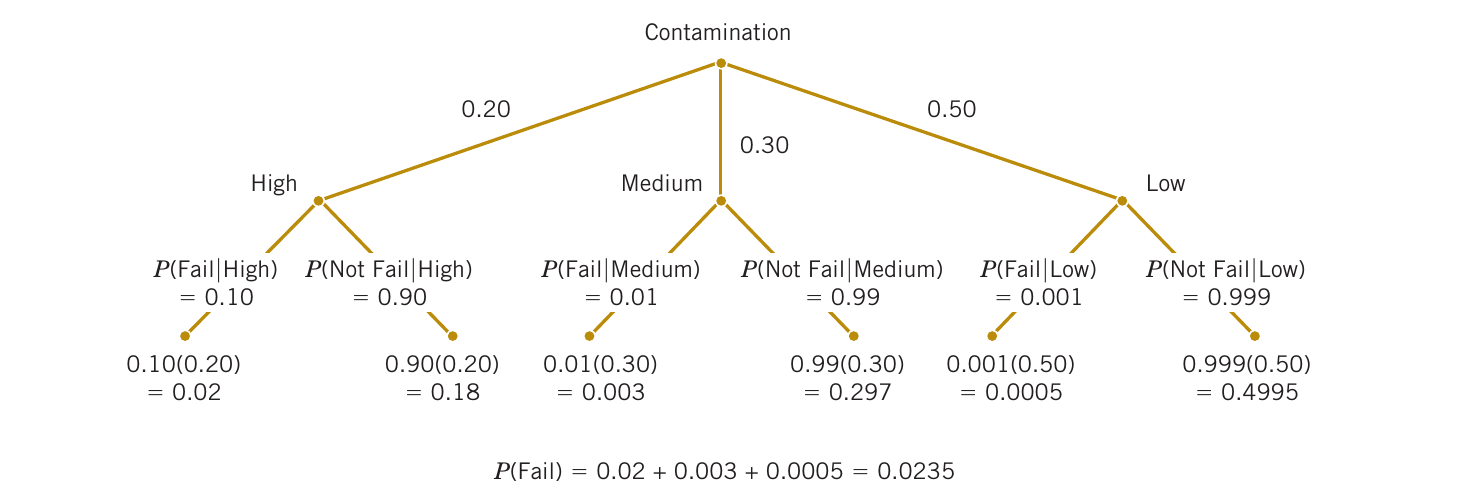
\includegraphics[scale=0.35]{2.png}
       \end{center}
     
   } 
  
\end{document}